%!TEX root = ../../master.tex
\noindent \textbf{Use Timeouts}
\\
The timeout pattern is concerned with the first fallacy about trusting the network blindly. The risk of blocking a thread forever and eventually draining a thread pool is present without timeouts. Slow responses can lead to cascading failures and chain reactions. The solution is to limit the acceptable waiting time and have a fallback strategy. Using the terms from Figure~\ref{fig:our_resilience_definition}, this is a way of prioritizing availability over reliability by tolerating a lower level of consistency. A lower level of consistency could be a degradation in the returned content e.g. returning a top10 movie list instead of a personalized list. \\

\noindent \textbf{Circuit Breaker}
\\
A circuit breaker protects a service from an unhealthy integration point by applying rules for when it is allowed to call the integration point. When an integration point fails too many times (e.g. timeout) it is blocked and transitions from the state \textit{closed} to \textit{open} (Figure~\ref{fig:circuit_breaker_states}). Given a configuration, the circuit breaker transitions to the \textit{half-open} state in which it attempts a reset its state to see if the integration point is safe to call again. If the attempt succeeds the state transitions from \textit{half-open} to \textit{closed}, and if the attempts fails it returns to the \textit{open} state.

\begin{figure}[H]
    \centering
    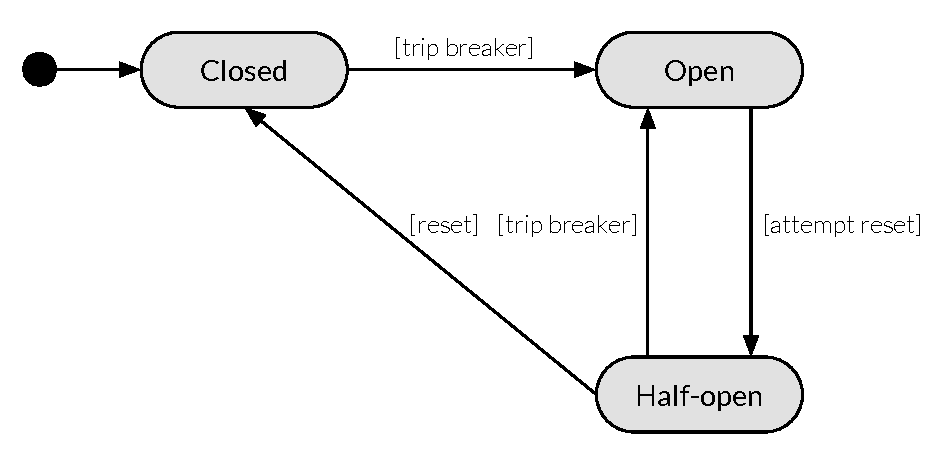
\includegraphics[width=10cm]{figures/circuit_breaker_state_diagram}
    \caption{Circuit Breaker States}
    \label{fig:circuit_breaker_states}
\end{figure}

\noindent 
Fallback methods can be used together with circuit breakers to degrade gracefully instead of failing. As with timeouts, this is trading higher availability at the cost of consistency and reliability. An experiment involving circuit breakers, fallback methods and avoidance of cascading failures is presented in Section~\ref{sec:exp_integration_points}. \\


\noindent \textbf{Fail Fast}
\\
The fail fast pattern summarizes the similarity in the two previous patterns. Failing slowly is worse than failing fast, and several antipatterns are linked to waiting. If services are synchronously chained (A calls B who calls C) much time may be wasted in the form of blocked threads. Timeouts and circuit breakers exemplify how this pattern can be implemented. \\

\noindent \textbf{Bulkheads}
\\
Another recurring theme in the previous patterns has been the containment of damage. In ships, bulkheads are used to contain damage to a certain part of a ship (Figure~\ref{fig:bulkheads}). 

\begin{figure}[H]
    \centering
    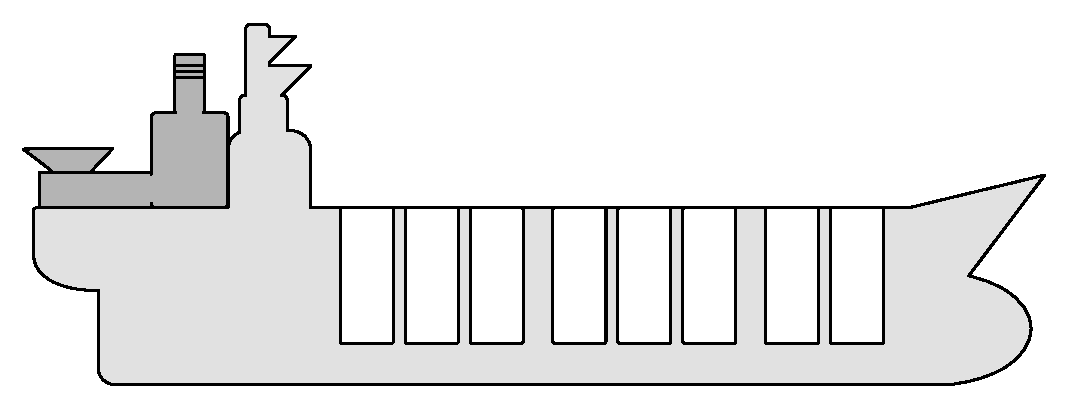
\includegraphics[width=10cm]{figures/bulkheads}
    \caption{Bulkheads}
    \label{fig:bulkheads}
\end{figure}

\noindent
Bulkheads can be applied at different levels. At the application level, the architecture can be split into multiple services such as microservices and gain the containment through multiple processes. 
When interacting with different integration points, different thread pools within the service can be used. The benefit comes with the price of less flexibility to share resources when one of the integration points is passive. \\

\noindent \textbf{Decoupling Middleware}
\\
Nygard describes different degrees of coupling in middleware and points out that some of the previously described problems can be mitigated by decoupling middleware. A step in this direction could e.g. be to choose a message queue instead of HTTP for communication between services.

\begin{citat} []
"Message-oriented middleware decouples the endpoints in both space and time. Because the requesting system doesn't just sit around waiting for a reply, this form of middleware cannot produce a cascading failure."\textbf{- Nygard, 2007} \cite[p. 115]{nygard2007release}
\end{citat}

\noindent Furthermore, Nygard states that synchronous (tightly coupled) middleware's advantage is \textit{"its logical simplicity"} opposite of asynchronous processes that are \textit{"inherently harder"} \cite[p. 115]{nygard2007release}. Newman points out the same increase in complexity in asynchronous programming. The inherent complexity will most likely result in an increase in Mansouri et al's \cite[p. 16]{omer2013resilience} disruption caused by a human factor.

\begin{citat} []
"The associated complexity with event-driven architectures and asynchronous programming in general leads me to believe that you should be cautions in how eagerly you start adopting these ideas." \textbf{- Newman, 2015} \cite[p. 57]{newman2015building}
\end{citat}

\noindent On the other hand, Bonér, the inventor of the Akka framework, expresses asynchronous communication as a requirement for isolation and, thereby, resilience.
\begin{citat} []
Isolation is a prerequisite for resilience and elasticity and requires asynchronous communication boundaries between services to decouple them in: Time (Allowing concurrency), Space (Allowing distribution - and mobility — the ability to move services around) \textbf{- Bonér, 2016} \cite[p. 7]{boner2016reactive}
\end{citat}

\noindent Throughout the rest of this master's thesis, the focus will primarily be on synchronous communication. The designed course (Chapter~\ref{chap:designing_learning_acitivty}) already contains many new concepts. Netflix is an example of a company using a synchronous architecture. However they have created a reactive extension called RxJava that introduces asynchronous behavior.